\documentclass[aspectratio=169]{beamer}
\usepackage{color,amsmath}
\usepackage{subfigure}
\usepackage{booktabs}
\usepackage{framed}
\usepackage{comment}
\usepackage{ulem}

\usepackage{hyperref}
\hypersetup{
    colorlinks=true,
    linkcolor=blue,
    filecolor=magenta,      
    urlcolor=cyan,
}



%%%%%%%%%%%%%%%%%%%%%%%%%%
\title[]{\textcolor{gray}{[Introduction to mass collaboration],} [Human computation], \textcolor{gray}{[Open call], [Distributed data collection], \newline [Fragile Families Challenge]}}
\author[]{Matthew J. Salganik\\Department of Sociology\\Princeton University}
\date[]{%Summer Institutes in Computational Social Science\\2020
%\vfill
%\begin{flushleft}
%{\scriptsize
%The Summer Institutes in Computational Social Science is supported by grants from the Russell Sage Foundation and the Alfred P. Sloan Foundation.}
%\end{flushleft}
\begin{flushright}

\includegraphics[width=0.1\textwidth]{figures/cc-by.png}
\end{flushright}
}
\begin{document}
%%%%%%%%%%%%%%%%%%%%%%%%%%
\frame{\titlepage}
%%%%%%%%%%%%%%%%%%%%%%%%%%
\begin{frame}

\begin{columns}
\begin{column}{.40\textwidth}

\includegraphics[width=\textwidth]{figures/salganik_bit_2018_cover}
\end{column}%

\hfill%

\begin{column}{.60\textwidth}
1) Introduction \\
2) Observing behavior \\
3) Asking questions \\
4) Running experiments \\
\textcolor{blue}{5) Mass collaboration} \\
6) Ethics \\
7) The future \\
\end{column}%
\end{columns}

\end{frame}
%%%%%%%%%%%%%%%%%%%%%%%%%
\begin{frame}

\begin{center}
\only<1>{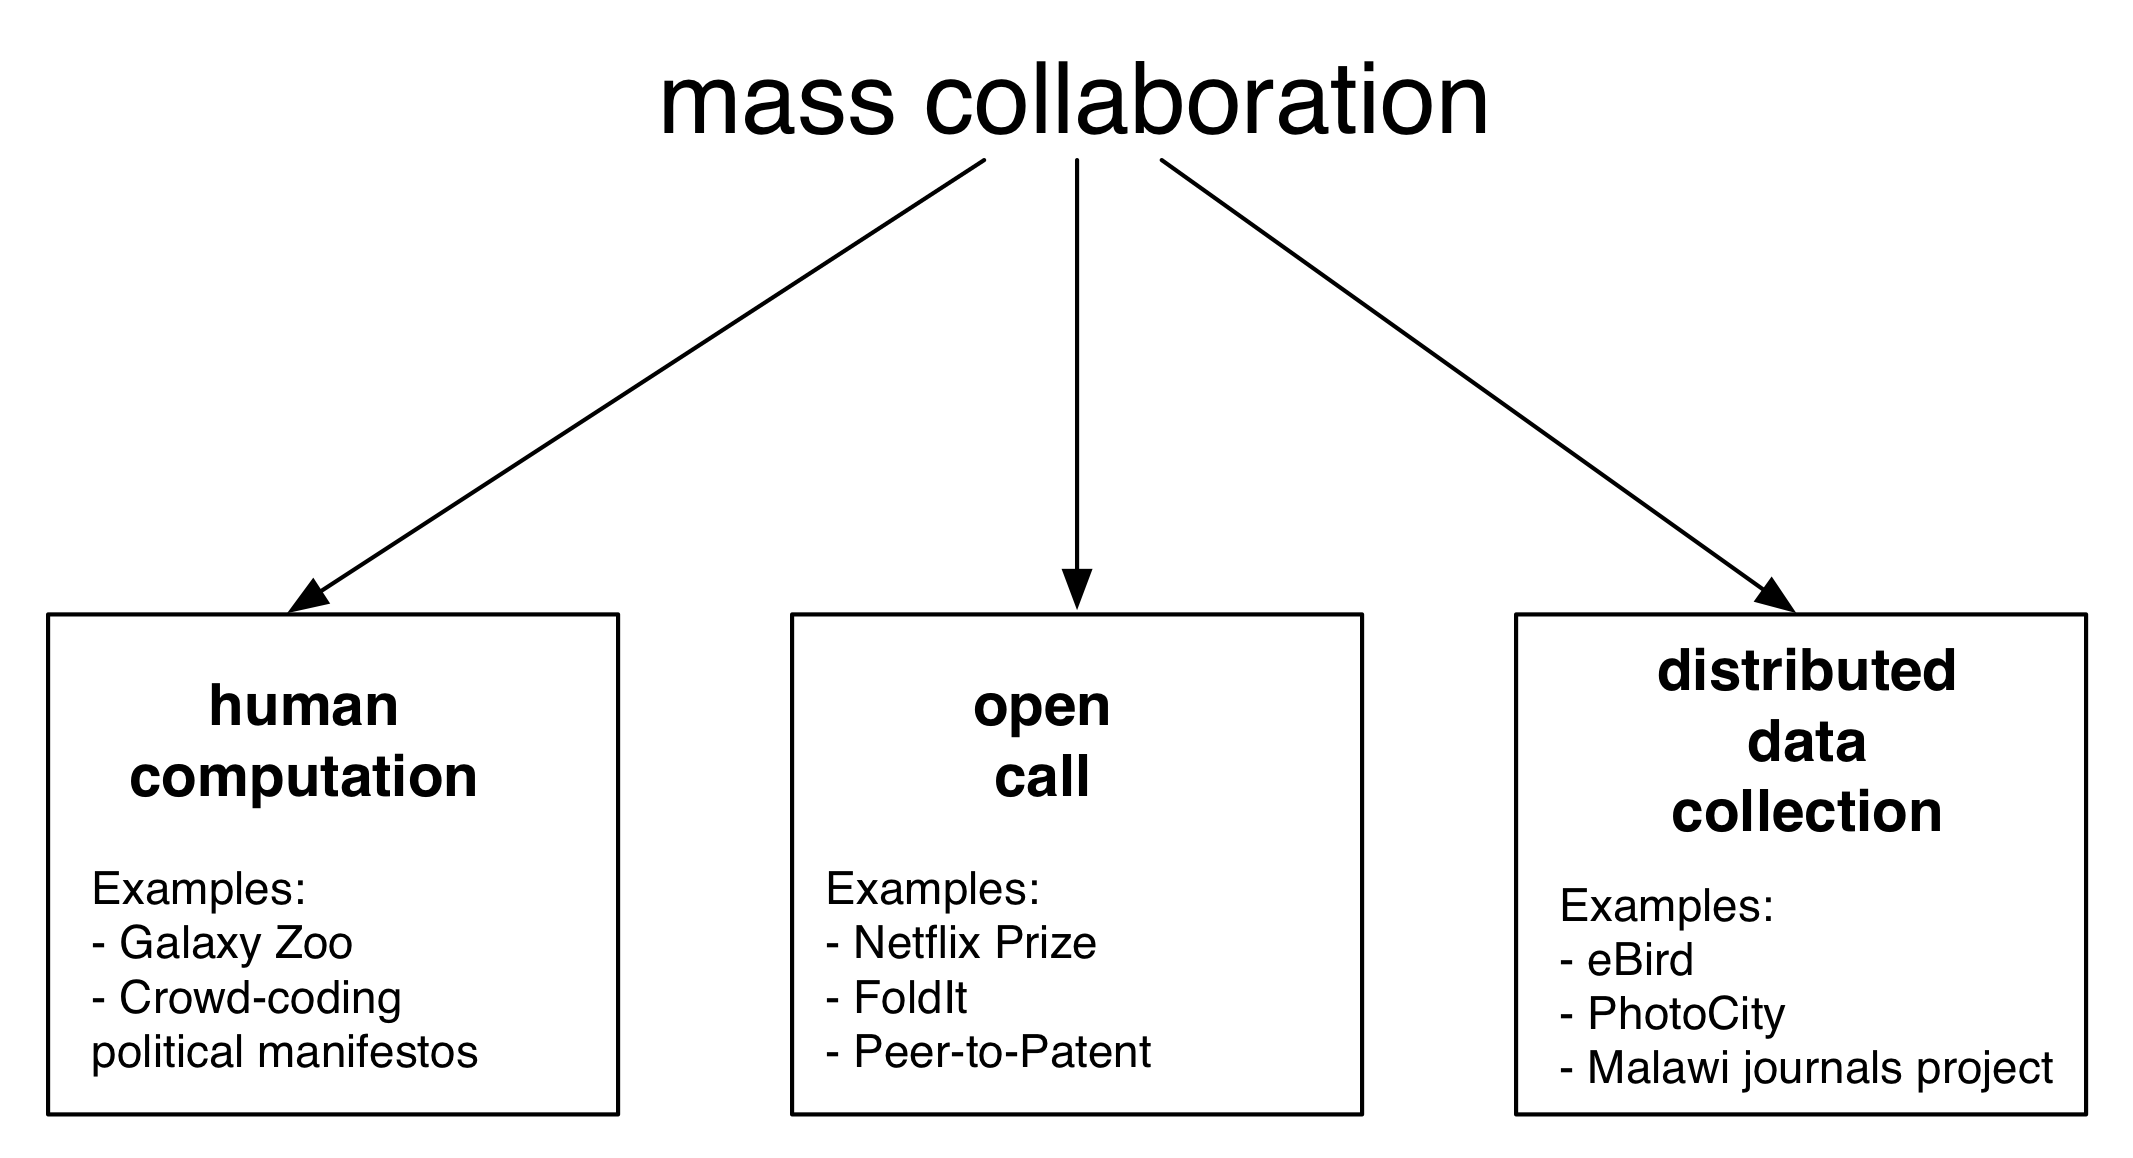
\includegraphics[width=0.9\textwidth]{figures/mass_collaboration_schematic}}
\only<2>{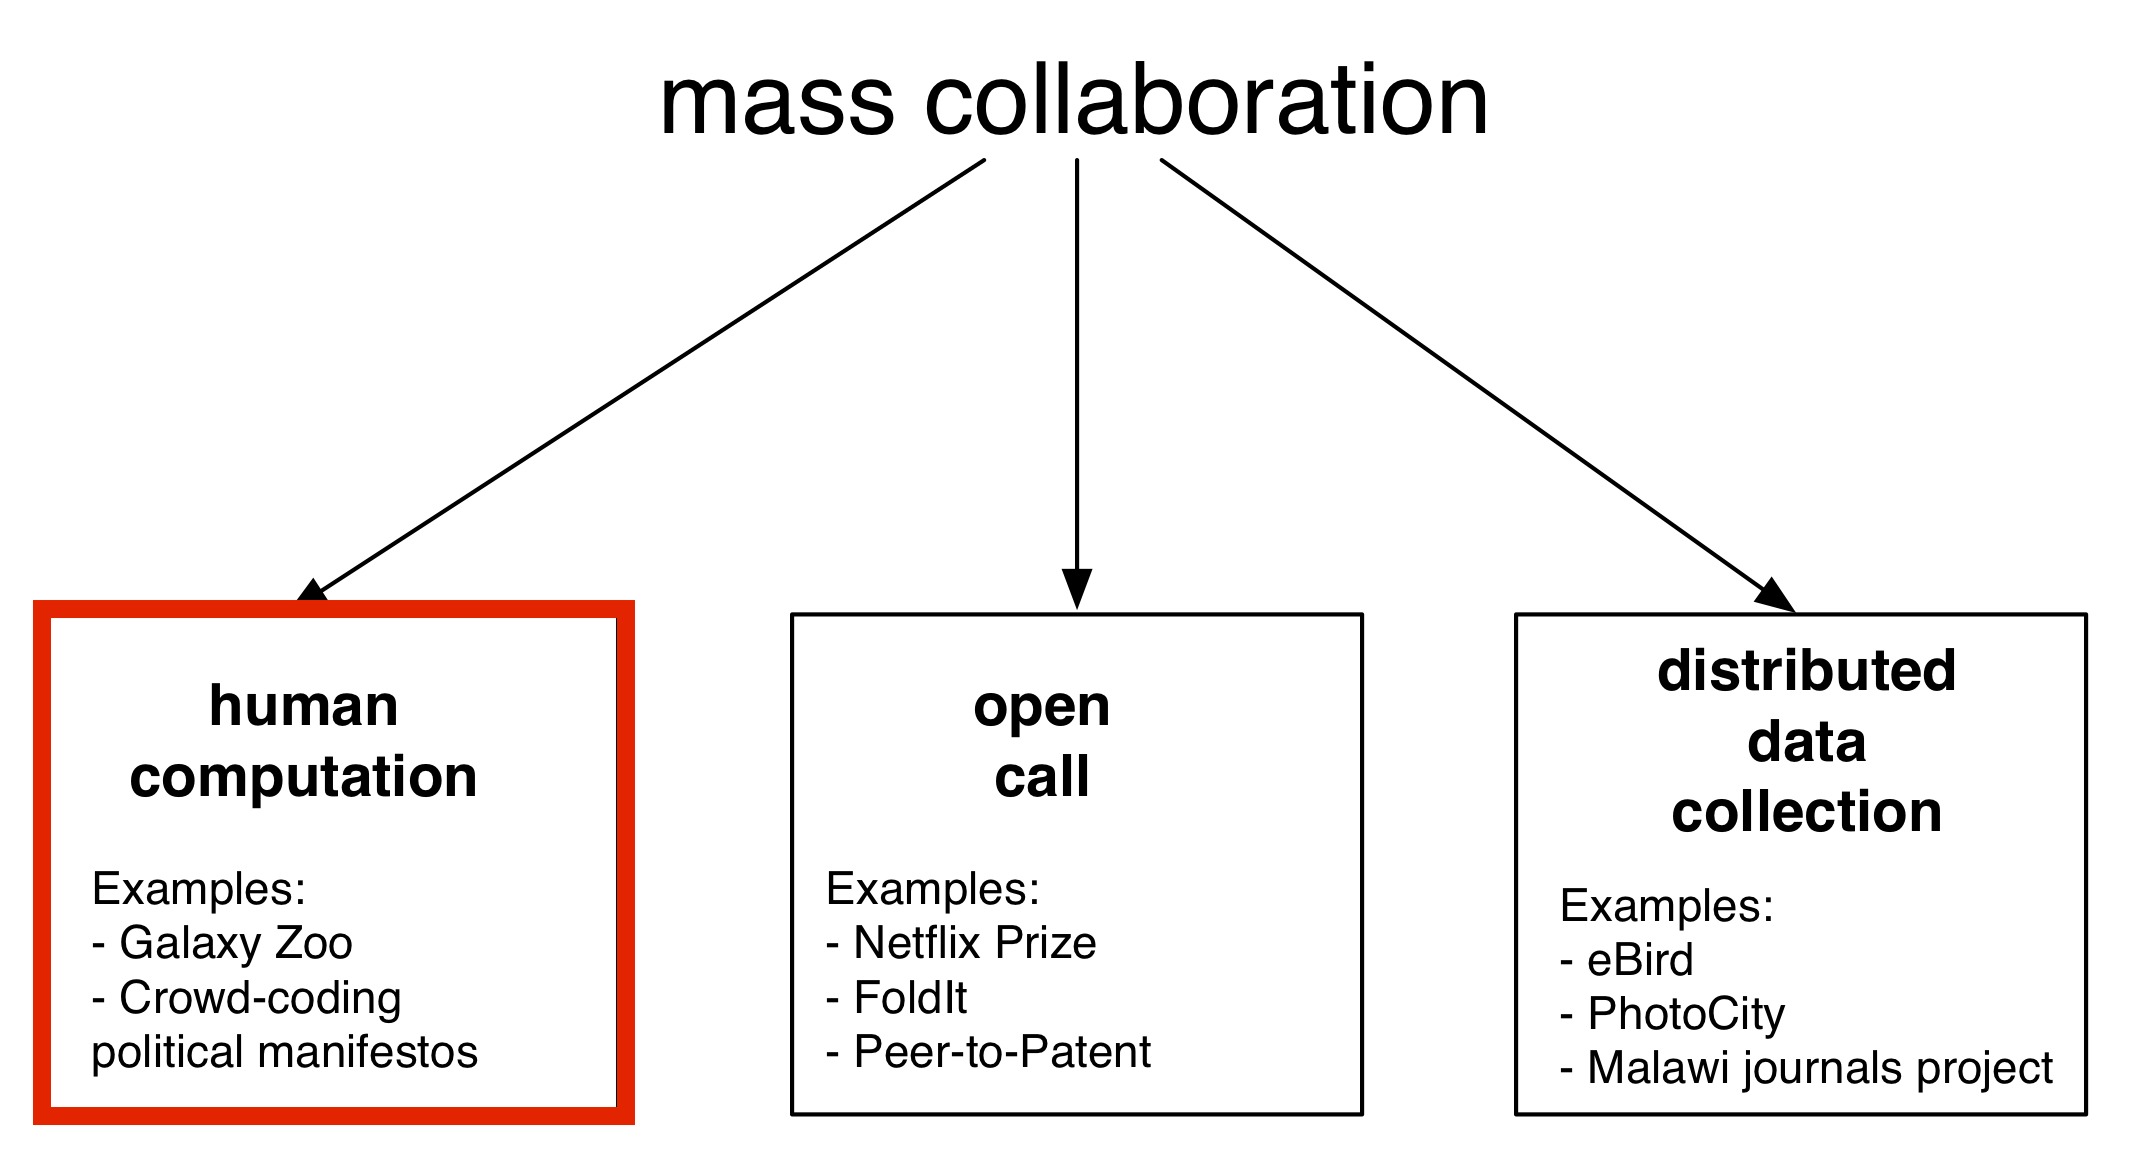
\includegraphics[width=0.9\textwidth]{figures/mass_collaboration_schematic_human_computation}}
\end{center}

\vfill
Fig 5.4 (\href{https://www.bitbybitbook.com/}{Salganik 2018})
\end{frame}
%%%%%%%%%%%%%%%%%%%%%%%%%%
\begin{frame}

Human computation:
\begin{itemize}
\item Easy task, big scale problems where humans better than computers
\pause
\item Split-apply-combine strategy
\pause
\item Human effort can be magnified with supervised learning 
\pause
\item Increasingly important as we move from numeric survey data to working with text, images, movies, and audio.
\end{itemize}

\end{frame}
%%%%%%%%%%%%%%%%%%%%%%%%%%
\begin{frame}
\frametitle{Galaxy Zoo}

Astronomers are interested in understanding the relationship between the shape and color of galaxies

\begin{figure}
  \centering
  \subfigure[Elliptical]{
  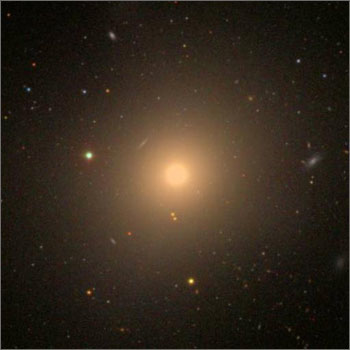
\includegraphics[width=0.40\textwidth]{figures/gz_example_elliptical}}
  \hspace{0in}
  \subfigure[Spiral]{
  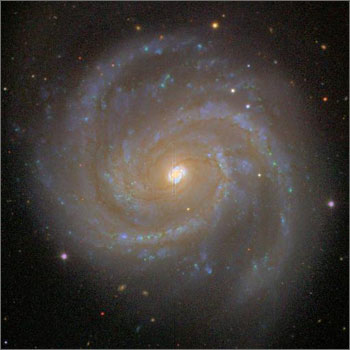
\includegraphics[width=0.40\textwidth]{figures/gz_example_face_on_spiral}}
\end{figure}

\end{frame}
%%%%%%%%%%%%%%%%%
\begin{frame}
\frametitle{Galaxy Zoo}

Needed hand-classified galaxies so Schwaninski worked seven, 12 hour days to classify 50,000 galaxies
\begin{center}
\fbox{
\includegraphics[width=\textwidth]{figures/schawinski_paper_2007}}
\end{center}
\pause
\vfill
Only 5\% of the $\sim1$ million galaxies in the Sloan Digital Sky Survey.  A new approach was needed . . . .
\end{frame}
%%%%%%%%%%%%%%%%%
\begin{frame}
\frametitle{}

\begin{center}
\includegraphics[width=0.8\textwidth]{figures/galaxy_zoo_input_screen}
\end{center}

\end{frame}
%%%%%%%%%%%%%%%%%
\begin{frame}
\frametitle{Galaxy Zoo}

\begin{itemize}
\item Volunteers had a $\sim$5 minute training and passed a quiz
\item Categorized as many or as few galaxies as they wished
\item Much of the recruiting happened through the media
\end{itemize}

\end{frame}
%%%%%%%%%%%%%%%%%
\begin{frame}
\frametitle{Galaxy Zoo}

\setcounter{subfigure}{0}
\begin{figure}
  \centering
  \subfigure[Classifications over time]{
  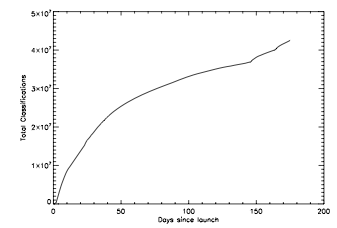
\includegraphics[width=0.54\textwidth]{figures/lintott_galaxy_2008_fig2}}
  \hspace{0.05\textwidth}
  \subfigure[Classifications per user]{
  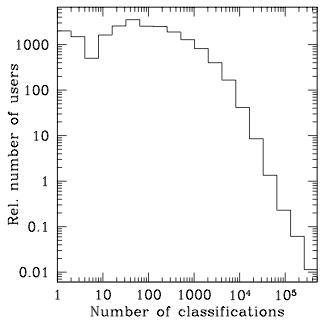
\includegraphics[width=0.36\textwidth]{figures/lintott_galaxy_2008_fig3}}
\end{figure}

\end{frame}
%%%%%%%%%%%%%%%%%
\begin{frame}
\frametitle{Galaxy Zoo}

40 million classification to a consensus labels (Lintott et al., 2011)
\begin{enumerate}
\item \textcolor{blue}{Cleaning} 
\begin{itemize}
\item only the first classification that a volunteer made of a specific galaxy was used in the analysis
\item anyone who classified more than 2 galaxies more than 5 times each had all their classifications discarded
\end{itemize}
\pause
\item \textcolor{blue}{De-biasing}
\begin{itemize}
\item bias to classify far away spiral galaxies as elliptical galaxies (Bamford et al., 2009)
\end{itemize}
\pause
\item \textcolor{blue}{Combining} ($\sim$40 classifications per galaxy)
\begin{itemize}
\item use classifier/classification matrix to upweight good classifiers 
\end{itemize}
\end{enumerate}
\vfill
Produces data comparable in quality to expert coders (Lintott et al. 2011), but at much greater scale

\end{frame}
%%%%%%%%%%%%%%%%%%%
\begin{frame}
\frametitle{Galaxy Zoo}

From millions to billions to trillions . . . .

\end{frame}
%%%%%%%%%%%%%%%%%%%
\begin{frame}
\frametitle{Galaxy Zoo}

\begin{center}
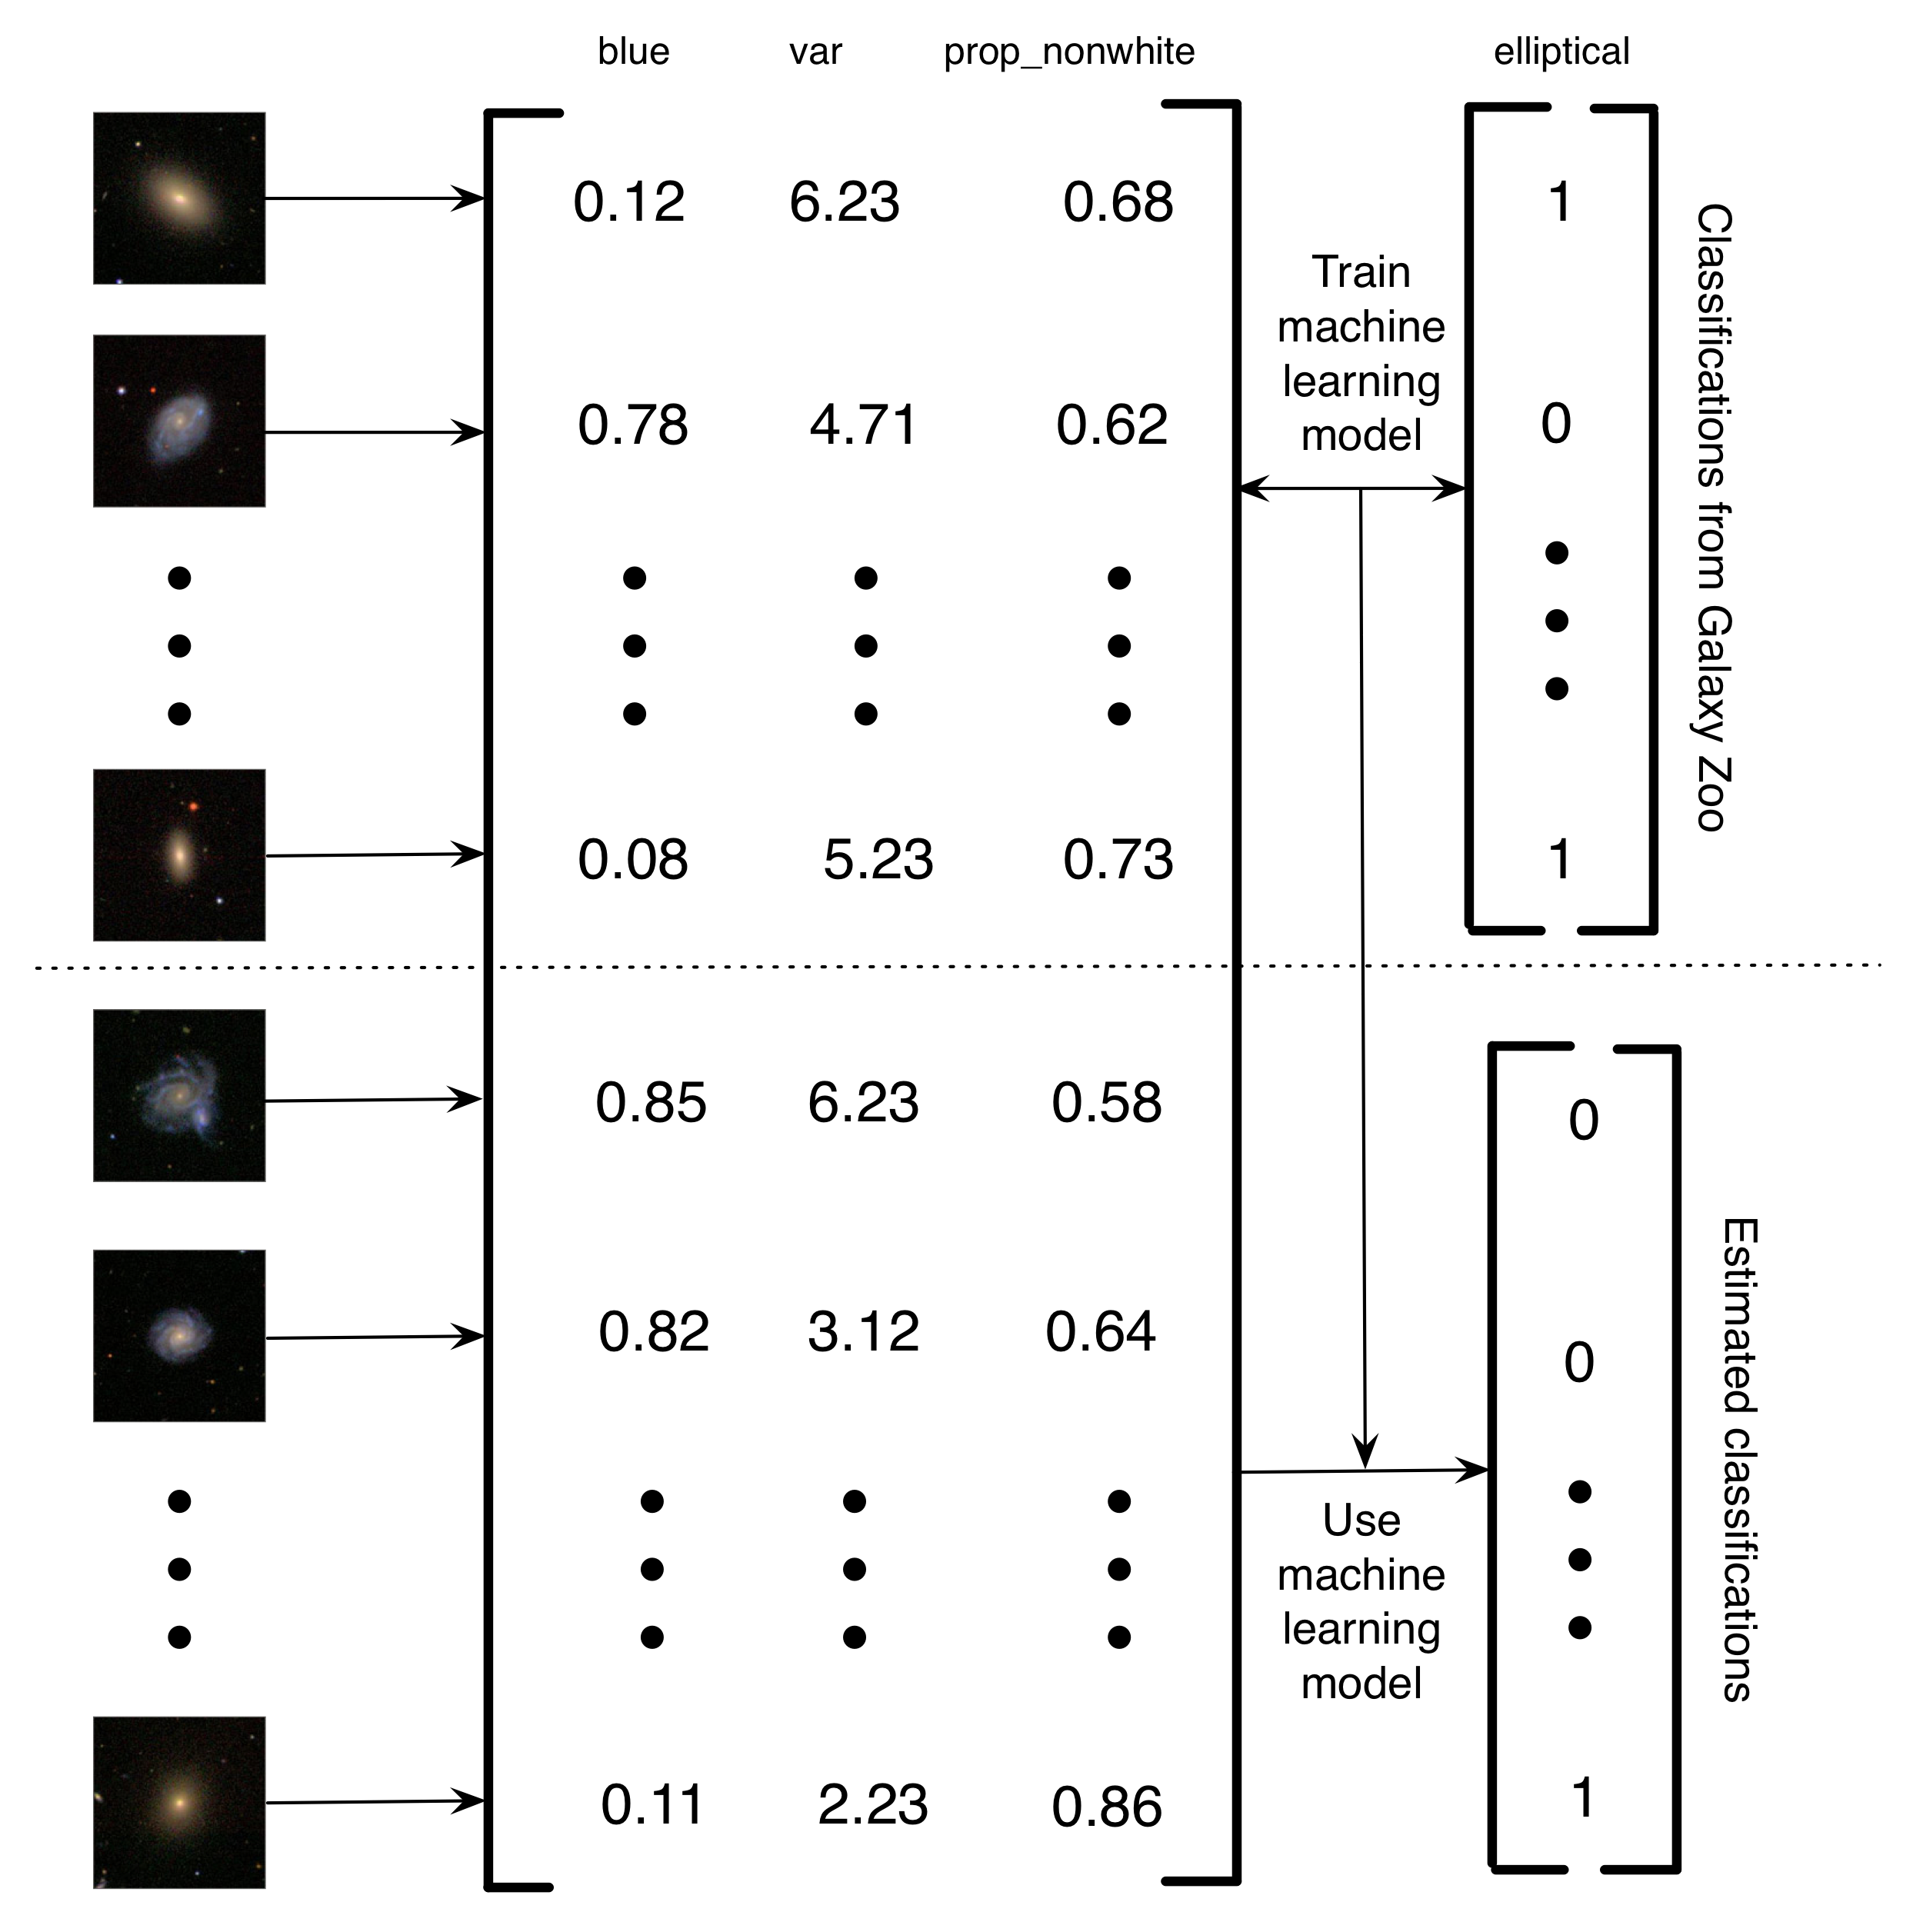
\includegraphics[height=0.8\textheight]{figures/bitbybit5-4_gz_banerji_schematic}
\end{center}

\vfill
Fig 5.4 (\href{https://www.bitbybitbook.com/}{Salganik 2018}), inspired by \href{https://doi.org/10.1111/j.1365-2966.2010.16713.x}{Banerji et al.\ (2010)}
\end{frame}
%%%%%%%%%%%%%%%%%%
\begin{frame}

\begin{center}

\includegraphics[width=\textwidth]{figures/zooniverse_logo}
\end{center}

\vfill
\url{https://www.zooniverse.org/}
\end{frame}
%%%%%%%%%%%%%%%%%%%%%%%%%%
\begin{frame}

\begin{center}
\only<1>{\includegraphics[width=\textwidth]{figures/benoit_crowd-sourced_2016_title}}
\only<2>{\includegraphics[width=\textwidth]{figures/benoit_crowd-sourced_2016_abstract}}
\end{center}

\vfill
\href{http://dx.doi.org/10.1017/S0003055416000058}{Benoit et al.\ (2016)}

\end{frame}
%%%%%%%%%%%%%%%%%%%%%%%%%%
\begin{frame}

Here's a piece of the manifesto of the Labor Party in the United Kingdom from 2010:

\begin{quote}
``Millions of people working in our public services embody the best values of Britain, helping empower people to make the most of their own lives while protecting them from the risks they should not have to bear on their own. Just as we need to be bolder about the role of government in making markets work fairly, we also need to be bold reformers of government.''
\end{quote}

\end{frame}
%%%%%%%%%%%%%%%%%%%%%%%%%%
\begin{frame}

\begin{center}
\only<1>{\includegraphics[width=\textwidth]{figures/benoit_crowd-sourced_2016_fig1}}
\only<2>{\includegraphics[width=\textwidth]{figures/benoit_crowd-sourced_2016_fig3}}
\end{center}

\end{frame}
%%%%%%%%%%%%%%%%%%%%%%%%%%
\begin{frame}

What I like about Benoit et al.\ (2016)
\begin{itemize}
\item Better not cheaper
\pause
\item Experts are a bug not a feature
\end{itemize}

\end{frame}
%%%%%%%%%%%%%%%%%%%%%%%%%%
\begin{frame}

Wrapping up:
\begin{itemize}
\item Easy task, big scale problems where humans better than computers
\pause
\item Split-apply-combine strategy
\pause
\item Human effort can be magnified with supervised learning 
\pause
\item Increasingly important as we move from numeric survey data to working with text, images, movies, and audio.
\end{itemize}

\end{frame}
%%%%%%%%%%%%%%%%%%%%%%%%%%
\begin{frame}

What to read next:
\begin{itemize}
\item \href{https://dl.acm.org/doi/book/10.5555/2049960}{\textit{Human computation}} (Law and von Ahn, 2011))
\item \href{https://dx.doi.org/10.1126/science.1160379}{reCAPTCHA} (von Ahn et al.\ 2008) 
\item Background about Amazon Mechanical Turk: \href{https://dx.doi.org/10.1126/science.352.6291.1263}{Bohannon 2016}
\end{itemize}

\end{frame}
%%%%%%%%%%%%%%%%%%%%%%%%%%
\frame{\titlepage}
%%%%%%%%%%%%%%%%%%%%%%%%%


\end{document}
